\section{Sistema de Hierarquia de Níveis}

O  utilizado código possui uma estrutura hierárquica de níveis aninhados, que serve para fornecer estrutura aos algorítimos de refinamento de malha adaptativa (\textit{AMR}) e \textit{multigrid} (cite trabalhos). Essa hierarquia de níveis é mostrada na Figura \ref{fig:hierarquia_de_niveis}. Cada um dos níveis possui resíduos das variáveis calculadas pelo multigrid ou campos vetoriais completos quando esses níveis pertencerem aos níveis físicos do AMR.

\begin{figure}[H]
    \centering
    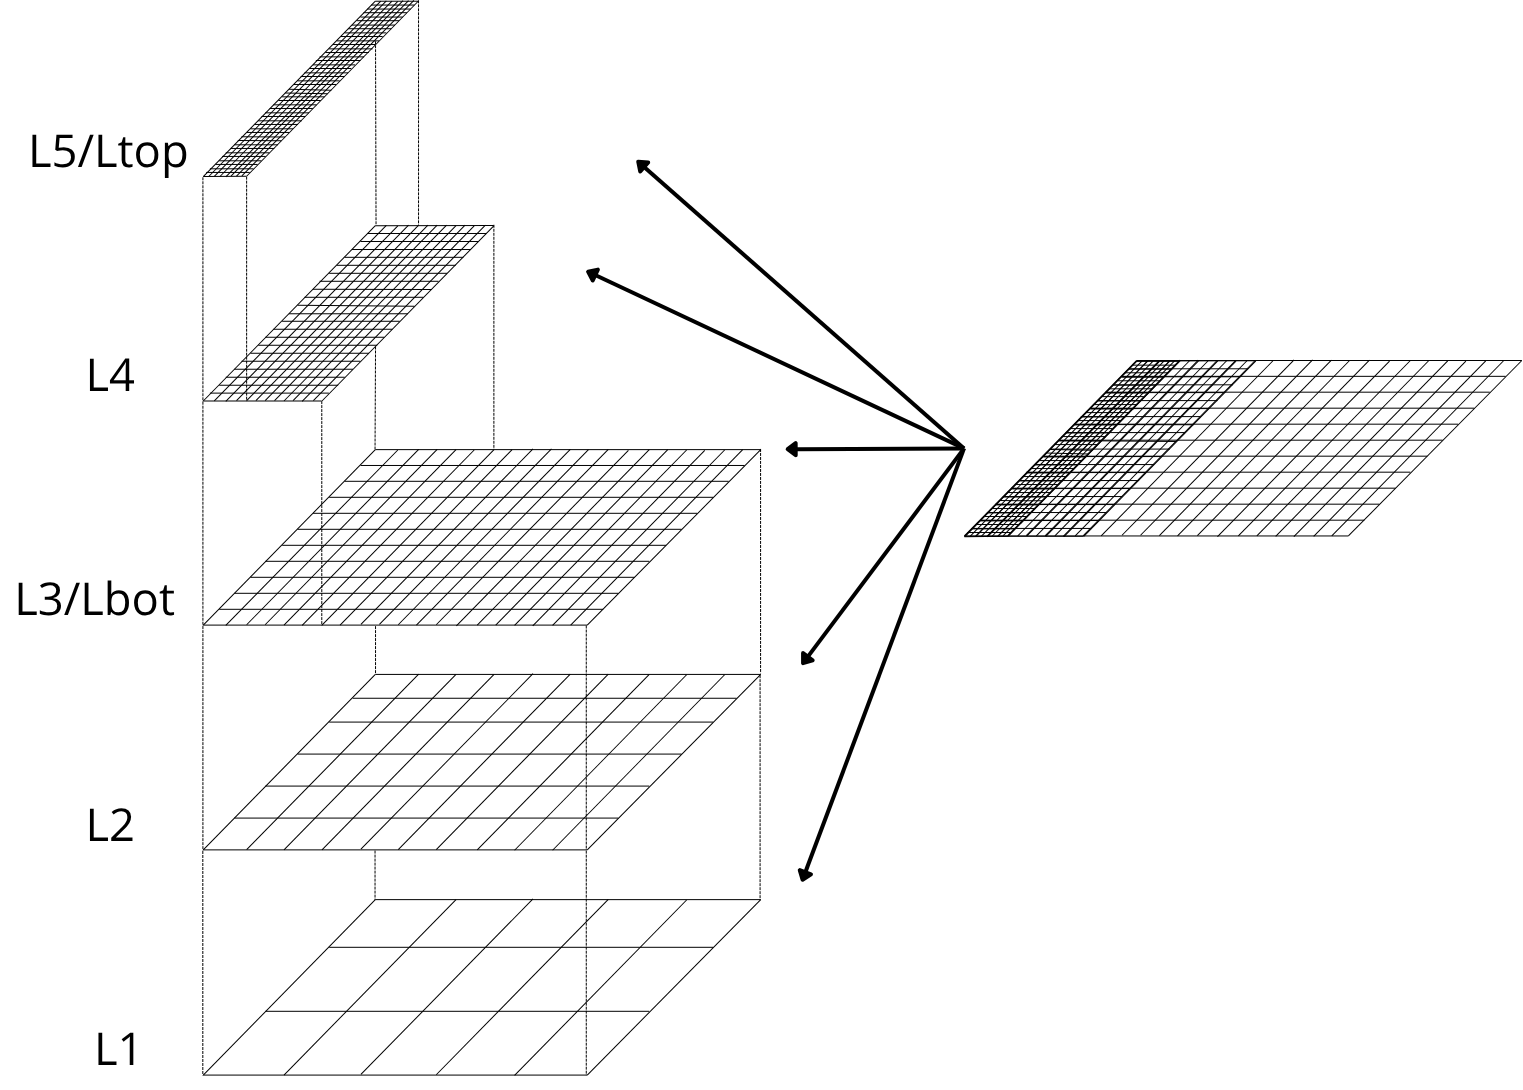
\includegraphics[width=0.7\textwidth]{imagens/estrutura_grid_mfsim.png}
    \caption{Esquema de como os níveis de malha se comportam no MFSim.}
    \label{fig:hierarquia_de_niveis}
\end{figure}

Tem-se então a divisão entre os níveis físicos, aqueles que resolvem o escoamento em si, os níveis intermediários que são apenas interpolados, e os níveis virtuais, que servem exclusivamente para a aplicação do método \textit{multigrid}. No exemplo da Figura \ref{fig:hierarquia_de_niveis} os níveis de L3 e L5 seriam os níveis físicos e os níveis L1 e L2 seriam apenas virtuais, tendo ainda o nível L4 que nesse contexto atuaria como nível intermediário.

Dessa forma, os níveis físicos guardam os campos, escalares e vetoriais, das propriedades físicas como: pressão, velocidade, e $f$ quando aplicável necessários para as interpolações do \textit{AMR} bem como os campos de resíduo e erro, necessários para a aplicação do \textit{multigrid}. Os níveis virtuais, porém, guardam apenas os campos resíduo e erro, sem terem informações dos campos vetoriais e escalares.


Dentro desta estrutura, os níveis físicos mais refinados resolvem suas condições de contorno a partir das condições globais, nas faces que encostam no limite do domínio, e a partir de interpolações de valores dos níveis inferiores nas faces que não tocam a fronteira do domínio.

Para o melhor entendimento da metodologia convenciona-se aqui \textit{ltop} o nível mais refinado da hierarquia multiníveis e como \textit{lbot} o último nível físico antes dos virtuais.

A metodologia proposta prevê confinar o escoamento bifásico no \textit{ltop}, assim sendo esse nível é "destacado" do ciclo de \textit{multigrid} e \textit{AMR} não sendo enxergado pelos demais, aos quais afeta de forma indireta. Nos níveis inferiores resolve-se o escoamento monofásico, sobre o qual são executados os ciclos e interpolações dos métodos mencionados sem a interferência do nível mais alto. Os níveis intermediários servem para guardar os campos, vindos dos níveis inferiores, para que sirvam de condição de contorno para o \textit{ltop}. A figura \ref{fig:hierarquia_metodo} mostra como a divisão funciona e o que roda em cada nível.

Os patches que pertencem ao \textit{ltop} estão sempre em contato, para pelo menos uma de suas faces, com a fronteira com o domínio ou com a fronteira imersa se utilizada e suas dimensões devem ser condizentes com a física esperada do filme, de forma que o fluido 1 esteja sempre confinado nos níveis mais finos da hierarquia. Apesar dos níveis inferiores não enxergarem diretamente o escoamento bifásico confinado, eles são influenciados pelo mesmo a partir das condições de contorno junto à parede que possui o filme.

\begin{figure}
    \centering
    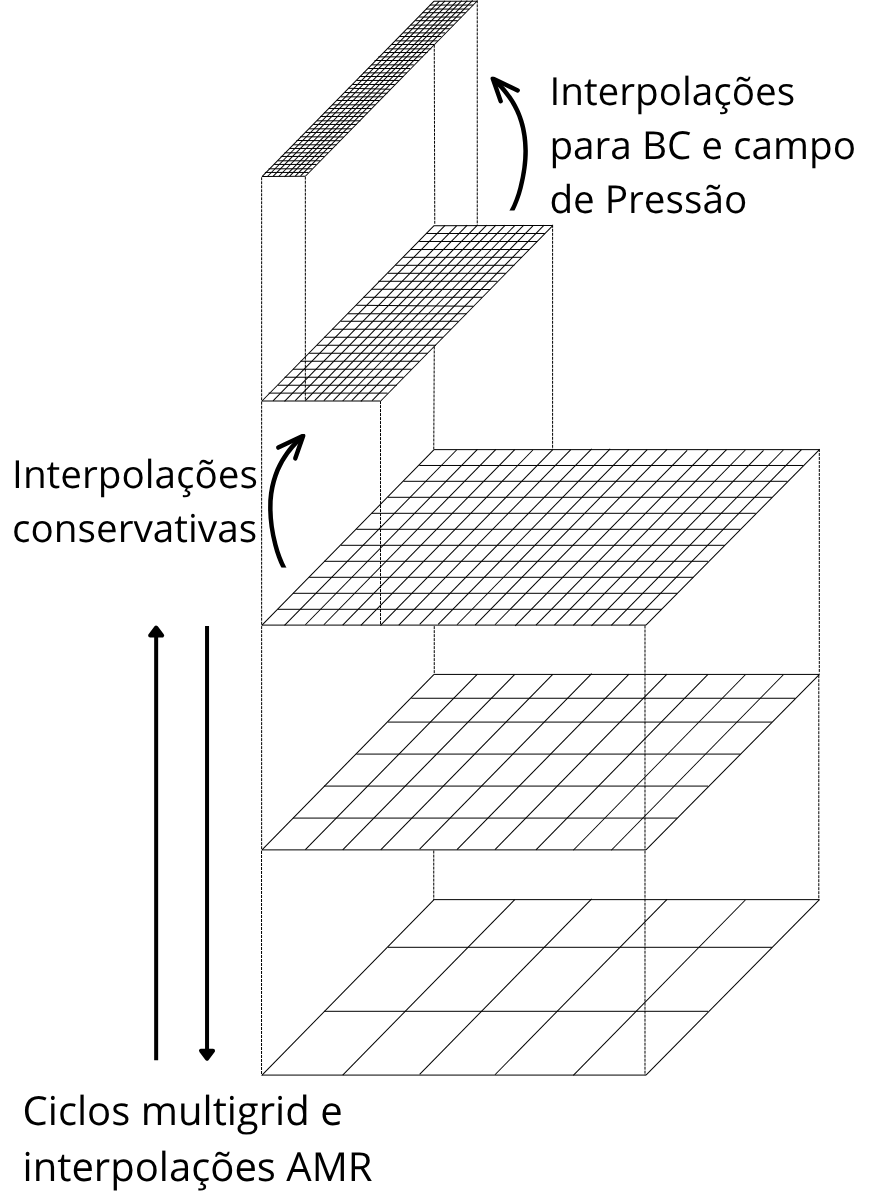
\includegraphics[width=0.7\textwidth]{imagens/hierarquia_de_interpolacoes.png}
    \caption{Esquema de como cada nível observa o outro e a direção na qual as interpolações são feitas.}
    \label{fig:hierarquia_metodo}
\end{figure}


